
\section{Actions}

\texttt{XmasAction}s in the UML Domain model diagram in appendix \ref{sec:Domain-Model-UML}
refers to the object type that performs actions inside the engine.
The reasoning behind these actions being its own class is to ensure
only one action at a time is being performed. This is because there
are many separate threads operating on the model code at once and
as such, there must be a way to active only one action at a time.

For the task of executing the actions we have the \texttt{ActionManager}.
Its job is to take in one action at a time and place them in a queue
(see fig. \ref{fig:ActionQueuing}).

\begin{figure}
\begin{centering}
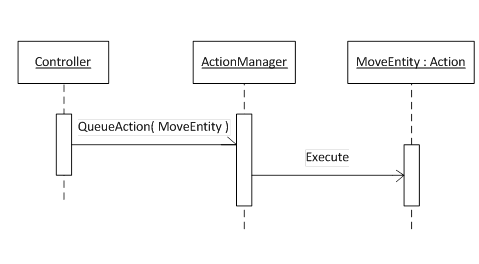
\includegraphics[width=0.7\textwidth]{ActionQueuing}
\par\end{centering}

\caption{\label{fig:ActionQueuing}Sequence diagram illustrating how a \texttt{MoveEntityAction}
is processed. The idea is that a controller, such as keyboard input
or an agent language, queues an action such as moving an entity on
the action manager. The action manager will then execute the action
as soon as it is ready.}
\end{figure}



\subsection{Action Types}

The engine is equipped with two different action types. One of them
is the \texttt{EnvironmentAction}, which are actions that perform
changes on the entire environment. Examples of such actions are closing
this engine or adding/removing entities from the world.

The other action type is the \texttt{EntityAction}. This action type
is meant as an action that a single entity performs; ideally the actions
should be as atomic as possible. In our reference implementation we
have given some ideas how these actions work, such as \texttt{grab},
which is an action that grabs a package from the tile the executing
agent is standing on.


\subsection{Example -- Move Entity Action}

Here we will show how an entity action is constructed by inheriting
the \texttt{EntityAction} class. As shown in fig. \ref{fig:MoveEntityActionExample},
we have created a \texttt{MoveEntityAction} class with one field containing
the direction of the move.

\begin{figure}
\begin{centering}
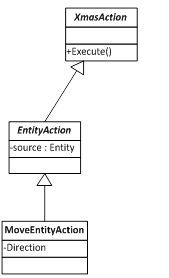
\includegraphics{MoveEntityActionExample}
\par\end{centering}

\caption{\label{fig:MoveEntityActionExample} Illustrating the inheritance
of the newly created \texttt{EntityAction} ``MoveEntityAction''}
\end{figure}


To have the action actually perform something, it is required that
an abstract method \texttt{Execute} is implemented. This execute method
is the method that is executed by the action manager. The implementation
of the execute action could then look something like the following
pseudo code:

\begin{alltt}
\textit{method} Execute \textit{returns} nothing 
    NewPosition = GetPositionOf(World, This.getSource()) + Direction 
    Wait(MOVE_TIME) 
    SetPositionOf(World,This.getSource(), NewPosition) 
\textit{EndMethod}
\end{alltt}

As one can see, the idea is that you find the position of the source
of the \texttt{EntityAction} and use that to generate the new position,
which is its old position incremented by its direction vector. The
wait is there to give the move a speed, as it would otherwise be an
instant movement.


\subsection{Summary}

Using actions is fairly simple and serves to shield the user from
the tedious and error prone workings that takes place behind the scenes.
It is meant to ensure thread safety and allow multiple threads working
with the engine at once. These were the exact reasons we chose this
design, as we ourselves had to deal with the problem of interference
from multiple concurrent threads. Furthermore, it will also reduce
code redundancy as generic actions can be reused by other actions.
The problem with this design is that it in a sense remakes what is
already implemented in a programming language. After all, running
procedural code is what programming languages are meant to do. However,
in return it provides a lot of utility and makes it possible to make
tools for simplifying the process of making actions. It also gives
the ability to differentiate between different action types and even
create new action types if one wishes so.
